%% Direttive TeXworks:
% !TeX root = ../../presentazione.tex
% !TEX encoding = UTF-8 Unicode
% !TEX program = arara
% !TEX TS-program = arara
% !TeX spellcheck = it-IT

\section{L'interfaccia classica}\label{sec:old}
\begin{frame}
    \frametitle{\insertsection}
    L'architettura di Alchemist è progettata con paradigma \engEmph{Model-View-Controller} (MVC), di conseguenza la suddivisione tra componente grafica (\engEmph{View}) e il blocco ``logico'' composto da \engEmph{Model} e \engEmph{Controller} è netta.

    \medskip
    \pause

    Questa distinzione è evidente anche per quanto riguarda l'utilizzo pratico del software:

    \begin{itemize}[<+(1)->]
      \item
          una simulazione su Alchemist può venire lanciata da terminale, senza che alcuna interfaccia grafica sia necessaria per tutta la durata del periodo di esecuzione \ldots

      \item
          \ldots oppure essere inizializzata, lanciata e controllata in tempo reale dalla sua interfaccia grafica.
    \end{itemize}
\end{frame}

\begin{frame}
    \frametitle{\insertsection}
    \centering
    \frame{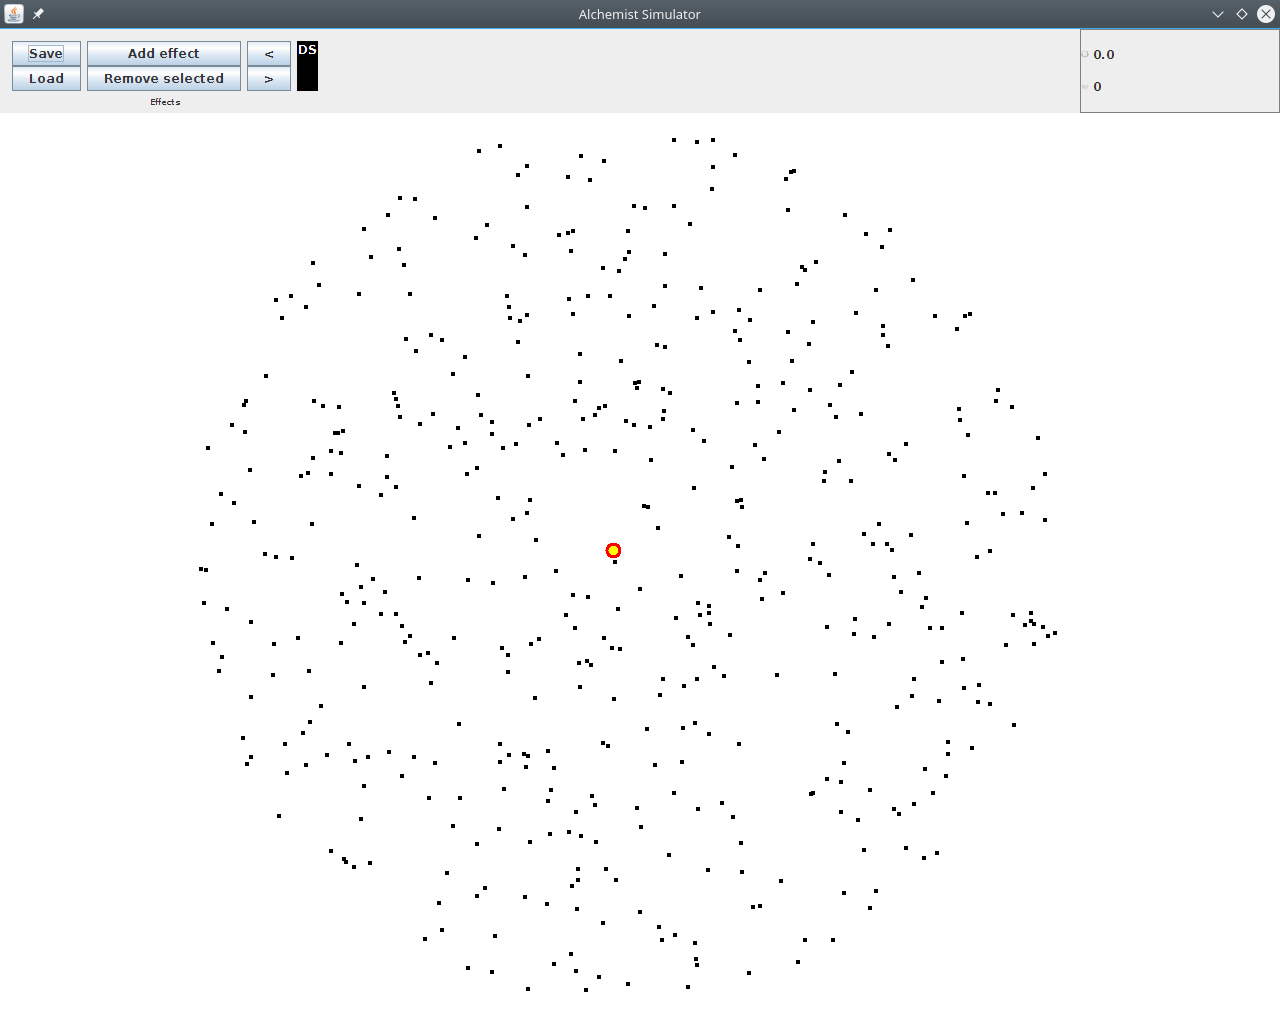
\includegraphics[scale=.29]{old/window_stopped_circle}}
\end{frame}

\begin{frame}
    \frametitle{\insertsection}

    L'interfaccia utente classica di Alchemist è caratterizzata da un'usabilità appena sufficiente, funzionale alle necessità di un utilizzatore esperto, ma non adeguata a fornire un'esperienza completa e \engEmph{user-friendly} ad un utente ``standard''.
    In particolare:

    \begin{itemize}[<+(1)->]
      \item
          Il sistema di controllo non è intuitivo: non sono presenti bottoni di interazione per, ad esempio, avviare o fermare la simulazione o per cambiare la modalità di interazione con la zona in cui viene rappresentato l'ambiente, bensì scorciatoie da tastiera.
      \item
          L'aspetto estetico è datato e non aderisce ad alcun design grafico conosciuto, né ne definisce uno proprio.
      \item
          Le capacità di rappresentazione, rappresentate dagli effetti, sono legate strettamente ai nodi e limitano la libertà di rappresentazione di ciò che avviene nella simulazione.
    \end{itemize}
\end{frame}
